  \section[Cloud]{Le Cloud : vue d'ensemble}

  \subsection[Cloud]{Le Cloud : les concepts}

  \begin{frame}
    \frametitle{Le cloud, c'est large !}
    \begin{itemize}
      \item Stockage/calcul distant \pause (on oublie, cf. externalisation)\pause
      \item Virtualisation++\pause
      \item Abstraction du matériel (voire plus)\pause
      \item Accès normalisé par des APIs\pause
      \item Service et facturation à la demande\pause
      \item Flexibilité, élasticité
    \end{itemize}
  \end{frame}

  \begin{frame}
    \frametitle{WaaS : Whatever as a Service}
    \begin{itemize}
      \item Principalement\pause
      \begin{description}
        \item[IaaS] \alert<5->{Infrastructure as a Service}\pause
        \item[PaaS] Platform as a Service\pause
        \item[SaaS] Software as a Service\pause
      \end{description}
      \pause
      \item Mais aussi :
      \pause
      \begin{itemize}
        \item Database as a Service
        \item Network as a Service
        \item Load balancing as a Service\pause
        \item \$APPLICATION as a Service
      \end{itemize}
    \end{itemize}
  \end{frame}

  \begin{frame}
    \frametitle{Cloud public ou cloud privé ?}
    \begin{description}
      \item[Public] fourni par un hébergeur à des clients (AWS, Rackspace Cloud, etc.)
      \item[Privé] plateforme et ressources internes
      \item[Hybride] utilisation de ressources publiques au sein d'un cloud privé
    \end{description}
  \end{frame}

  \begin{frame}
    \frametitle{Le cloud en un schéma}
    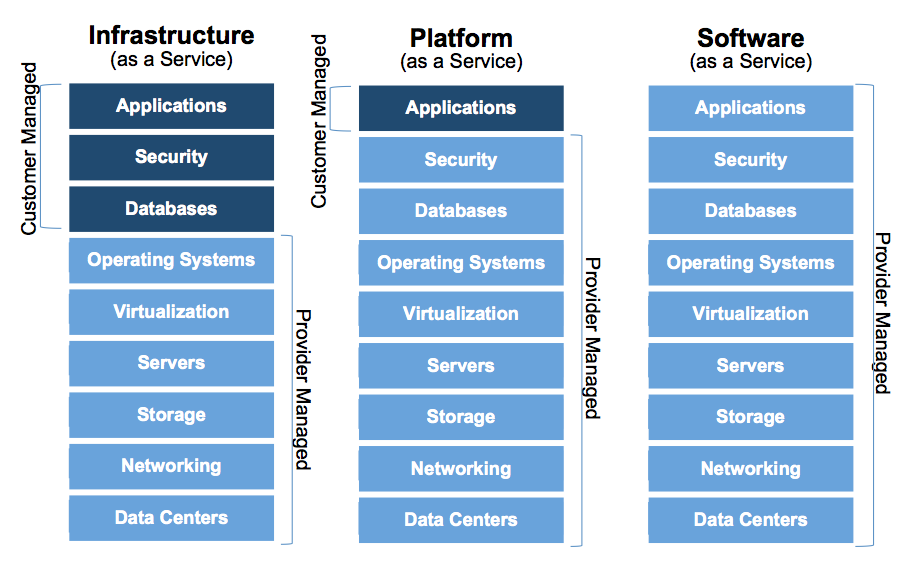
\includegraphics[width=\linewidth,height=\textheight]{images/cloud.png}
  \end{frame}

  \begin{frame}
    \frametitle{Pourquoi du cloud ? Côté business}
    \begin{itemize}
      \item Baisse des coûts par la mutualisation des ressources
      \item Utilisation uniquement des ressources qui sont nécessaires
      \item Va de pair avec l'automatisation du SI, l'agilité
      \item Donc réduction des délais et reproductibilité
      \item À grande échelle et/ou en cloud hybride, garantie de service
    \end{itemize}
  \end{frame}

  \begin{frame}
    \frametitle{Pourquoi du cloud ? Côté technique}
    \begin{itemize}
      \item Abstraction des couches plus basses
      \item On peut tout programmer à son gré
      \item Permet la mise en place d'architectures scalables
    \end{itemize}
  \end{frame}

  \subsection[PaaS]{PaaS : Platform as a Service}

  \begin{frame}
    \frametitle{PaaS : les principes}
    \begin{itemize}
      \item Fourniture d'une plateforme de développement
      \item Fourniture d'une plateforme de déploiement
      \item Pour un langage / un framework
      \item Principalement utilisé par des développeurs
    \end{itemize}
  \end{frame}

  \begin{frame}
    \frametitle{Exemples de PaaS publics}
    \begin{itemize}
      \item Amazon OpsWork / Elastic Beanstalk
      \item Google App Engine
      \item Heroku
    \end{itemize}
  \end{frame}

  \begin{frame}
    \frametitle{Solutions de PaaS privé}
    \begin{itemize}
      \item Cloud Foundry
      \item OpenShift (Red Hat)\pause
      \item Solum
    \end{itemize}
  \end{frame}

  \subsection[IaaS]{IaaS : Infrastructure as a Service}

  \begin{frame}
    \frametitle{Amazon Web Services (AWS) et les autres}
    \begin{itemize}
      \item Service (cloud public) : \textcolor{blue}{AWS}
      \begin{itemize}
        \item Pionnier du genre (dès 2006)\pause
        \item Elastic Compute Cloud (\textcolor{blue}{EC2})
        \item Elastic Block Storage (\textcolor{blue}{EBS})\pause
        \item Simple Storage Service (\textcolor{blue}{S3})\pause
      \end{itemize}
        \item Logiciels libres permettant le déploiement d'un cloud privé :
      \begin{itemize}
        \item Eucalyptus
        \item CloudStack
        \item OpenNebula\pause
        \item \textbf{OpenStack}
      \end{itemize}
    \end{itemize}
  \end{frame}

  \begin{frame}
    \frametitle{Les clouds publics concurrents d'AWS}
    \begin{itemize}
      \item Google Compute Platform
      \item Microsoft Azure
      \item \textbf<3->{Rackspace}
      \item \textbf<3->{HP Cloud}\pause
      \item En France
      \begin{itemize}
        \item \textbf<3->{Cloudwatt}
        \item \textbf<3->{Numergy}
        \item Outscale
        \item \textbf<3->{OVH}
        \item Ikoula
        \item \textbf<3->{Scaleway (Iliad)}
      \end{itemize}
    \end{itemize}
  \end{frame}

  \begin{frame}
    \frametitle{Virtualisation dans le cloud}
    \begin{itemize}
      \item Le cloud IaaS repose souvent sur la virtualisation
      \item Ressources compute $\leftarrow$ virtualisation
      \item Virtualisation complète : KVM, Xen
      \item Virtualisation containers : OpenVZ, LXC, Docker
    \end{itemize}
  \end{frame}

  \begin{frame}
    \frametitle{Notions et vocabulaire IaaS}
    \begin{itemize}
      \item Images
      \item Instances
      \item Types d'instance / gabarits (flavors)
      \item Volumes\pause
      \item Stockage block
      \item Stockage objet\pause
      \item IP flottantes/élastiques\pause
      \item Groupes de sécurité\pause
      \item Paires de clés\pause
      \item Templates, stacks\pause
      \item API REST\pause
      \item API de metadata et user data
      \item cloud-init, cloud-config
    \end{itemize}
  \end{frame}

  \begin{frame}
    \frametitle{Notions et vocabulaire IaaS}
    \begin{itemize}
      \item L'instance est par définition éphémère
      \item Elle doit être utilisée comme ressource de calcul
      \item Une image se personnalise lors de son instanciation grâce à l'API de metadata
      \item Séparer les données des instances
      \item Choix du type de stockage : éphémère, volume, objet
    \end{itemize}
  \end{frame}

  \begin{frame}
    \frametitle{À retenir}
    \Huge{Virtualisation $\ne$ IaaS}
  \end{frame}

  \begin{frame}
    \frametitle{AWS}
    \huge{Regardons l'interface web d'Amazon}
  \end{frame}

  \subsection[Stockage]{Stockage : block, objet, SDS}

  \begin{frame}
    \frametitle{Stockage block}
    \begin{itemize}
      \item Accès à des raw devices type \textit{/dev/vdb}
      \item Possibilité d'utiliser n'importe quel système de fichiers
      \item Compatible avec toutes les applications legacy
    \end{itemize}
  \end{frame}

  \begin{frame}
    \frametitle{Stockage objet}
    \begin{itemize}
      \item Pousser et retirer des objets dans un container/bucket
      \item Pas de hiérarchie des données, pas de système de fichiers
      \item Accès par les APIs
      \item L'application doit être conçue pour tirer partie du stockage objet
    \end{itemize}
  \end{frame}

  \begin{frame}
    \frametitle{Stockage objet : schéma}
    \begin{center}
      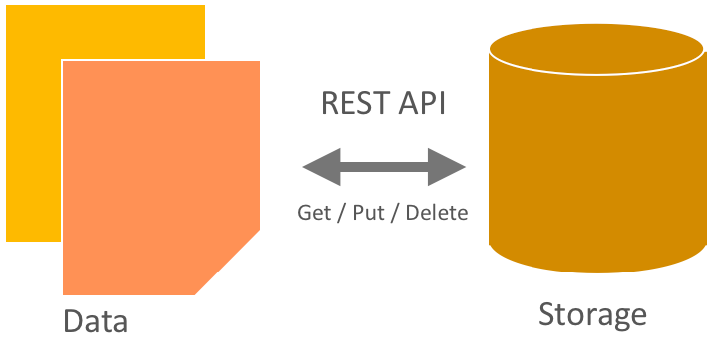
\includegraphics{images/stockage-objet.png}
    \end{center}
  \end{frame}

  \begin{frame}
    \frametitle{SDS : Software Defined Storage}
    \begin{itemize}
      \item Utilisation de commodity hardware
      \item Pas de RAID matériel
      \item Le logiciel est responsable de garantir les données
      \item Les pannes matérielles sont prises en compte et gérées
    \end{itemize}
  \end{frame}

  \begin{frame}
    \frametitle{Deux solutions : OpenStack Swift et Ceph}
    \begin{itemize}
      \item Swift fait partie du projet OpenStack et fournit du stockage objet
      \item Ceph fournit du stockage objet, block et FS
      \item Les deux sont implémentés en SDS\pause
      \item Théorème CAP : on en choisit deux
    \end{itemize}
  \end{frame}

  \begin{frame}
  \frametitle{Théorème CAP}
  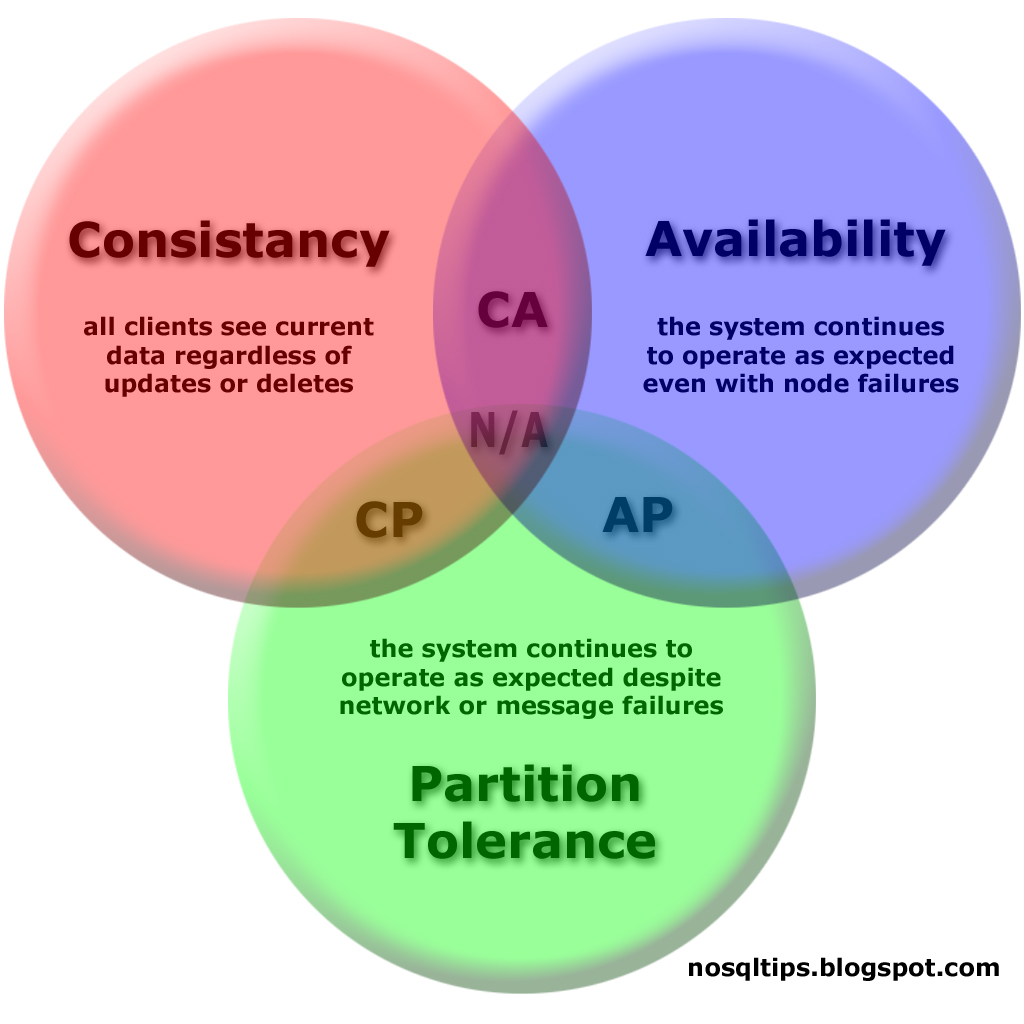
\includegraphics[width=\textwidth,height=\textheight]{images/cap.jpg}
  \end{frame}

  \begin{frame}
  \frametitle{Swift}
    \begin{itemize}
      \item Swift est un projet OpenStack
      \item Le projet est né chez Rackspace avant la création d'OpenStack
      \item Swift est en production chez Rackspace depuis lors
      \item C'est le composant le plus mature d'OpenStack
    \end{itemize}
  \end{frame}

  \begin{frame}
  \frametitle{Ceph}
    \begin{itemize}
      \item Projet totalement parallèle à OpenStack
      \item Supporté par une entreprise (Inktank) récemment rachetée par Red Hat
      \item Fournit d'abord du stockage objet
      \item L'accès aux données se fait via RADOS :
      \begin{itemize}
        \item Accès direct depuis une application avec librados
        \item Accès via une API REST grâce à radosgw
      \end{itemize}
      \item La couche RBD permet d'accéder aux données en mode block (volumes)
      \item CephFS permet un accès par un système de fichiers POSIX
    \end{itemize}
  \end{frame}

  \subsection[Orchestration]{Orchestrer les ressources de son IaaS}

  \begin{frame}
    \frametitle{Pourquoi orchestrer}
    \begin{itemize}
      \item Définir tout une infrastructure dans un seul fichier texte
      \item Être en capacité d'instancier une infrastructure entière en un appel API
      \item Autoscaling
      \begin{itemize}
        \item Adapter ses ressources en fonction de ses besoins en temps réel
        \item Fonctionnalité incluse dans le composant d'orchestration d'OpenStack
      \end{itemize}
    \end{itemize}
  \end{frame}

  \subsection[APIs]{APIs : quel rôle ?}

  \begin{frame}
    \frametitle{API ?}
    \begin{itemize}
      \item \textit{Application Programming Interface}
      \item Au sens logiciel : Interface permettant à un logiciel d'utiliser une bibliothèque
      \item Au sens cloud : Interface permettant à un logiciel d'utiliser un service (XaaS)
      \item Il s'agit le plus souvent d'API HTTP REST
    \end{itemize}
  \end{frame}

  \begin{frame}[containsverbatim]
    \frametitle{Exemple concret}
\begin{verbatim}
GET /v2.0/networks/<network_id>
{
   "network":{
      "status":"ACTIVE",
      "subnets":[
         "54d6f61d-db07-451c-9ab3-b9609b6b6f0b"
      ],
      "name":"private-network",
      "provider:physical_network":null,
      "admin_state_up":true,
      "tenant_id":"4fd44f30292945e481c7b8a0c8908869",
      "provider:network_type":"local",
      "router:external":true,
      "shared":true,
      "id":"d32019d3-bc6e-4319-9c1d-6722fc136a22",
      "provider:segmentation_id":null
   }
}
\end{verbatim}
  \end{frame}

